% Options for packages loaded elsewhere
\PassOptionsToPackage{unicode}{hyperref}
\PassOptionsToPackage{hyphens}{url}
\documentclass[
]{ltjsarticle}
\usepackage{xcolor}
\usepackage{amsmath,amssymb}
\setcounter{secnumdepth}{-\maxdimen} % remove section numbering
\usepackage{iftex}
\ifPDFTeX
  \usepackage[T1]{fontenc}
  \usepackage[utf8]{inputenc}
  \usepackage{textcomp} % provide euro and other symbols
\else % if luatex or xetex
  \usepackage{unicode-math} % this also loads fontspec
  \defaultfontfeatures{Scale=MatchLowercase}
  \defaultfontfeatures[\rmfamily]{Ligatures=TeX,Scale=1}
\fi
\usepackage{lmodern}
\ifPDFTeX\else
  % xetex/luatex font selection
\fi
% Use upquote if available, for straight quotes in verbatim environments
\IfFileExists{upquote.sty}{\usepackage{upquote}}{}
\IfFileExists{microtype.sty}{% use microtype if available
  \usepackage[]{microtype}
  \UseMicrotypeSet[protrusion]{basicmath} % disable protrusion for tt fonts
}{}
\makeatletter
\@ifundefined{KOMAClassName}{% if non-KOMA class
  \IfFileExists{parskip.sty}{%
    \usepackage{parskip}
  }{% else
    \setlength{\parindent}{0pt}
    \setlength{\parskip}{6pt plus 2pt minus 1pt}}
}{% if KOMA class
  \KOMAoptions{parskip=half}}
\makeatother
\usepackage{graphicx}
\makeatletter
\newsavebox\pandoc@box
\newcommand*\pandocbounded[1]{% scales image to fit in text height/width
  \sbox\pandoc@box{#1}%
  \Gscale@div\@tempa{\textheight}{\dimexpr\ht\pandoc@box+\dp\pandoc@box\relax}%
  \Gscale@div\@tempb{\linewidth}{\wd\pandoc@box}%
  \ifdim\@tempb\p@<\@tempa\p@\let\@tempa\@tempb\fi% select the smaller of both
  \ifdim\@tempa\p@<\p@\scalebox{\@tempa}{\usebox\pandoc@box}%
  \else\usebox{\pandoc@box}%
  \fi%
}
% Set default figure placement to htbp
\def\fps@figure{htbp}
\makeatother
\setlength{\emergencystretch}{3em} % prevent overfull lines
\providecommand{\tightlist}{%
  \setlength{\itemsep}{0pt}\setlength{\parskip}{0pt}}
\usepackage{bookmark}
\IfFileExists{xurl.sty}{\usepackage{xurl}}{} % add URL line breaks if available
\urlstyle{same}
\hypersetup{
  hidelinks,
  pdfcreator={LaTeX via pandoc}}

\author{}
\date{}

\begin{document}

\section{広がり位相を持つ二粒子の干渉------相対配置の特徴点と統計的対応の観察（観察論文・草案）}\label{ux5e83ux304cux308aux4f4dux76f8ux3092ux6301ux3064ux4e8cux7c92ux5b50ux306eux5e72ux6e09ux76f8ux5bfeux914dux7f6eux306eux7279ux5fb4ux70b9ux3068ux7d71ux8a08ux7684ux5bfeux5fdcux306eux89b3ux5bdfux89b3ux5bdfux8ad6ux6587ux8349ux6848}

\textbf{著者}：木原 範昭（Noriaki Kihara） \textbf{所属}：WF System Co.,
Ltd.~/ 大阪大学基礎工学部（卒業）
\textbf{ORCID}：\href{https://orcid.org/0009-0004-6753-4020}{0009-0004-6753-4020}
\textbf{版}：v1.0（公開候補・未査読） \textbf{日付}：2026 年 6 月
\textbf{ライセンス}：CC BY 4.0 \textbf{Concept
DOI}：\href{https://doi.org/10.5281/zenodo.20544004}{10.5281/zenodo.20544004}
\textbf{Version DOI
(v1.0)}：\href{https://doi.org/10.5281/zenodo.20544005}{10.5281/zenodo.20544005}

\begin{center}\rule{0.5\linewidth}{0.5pt}\end{center}

\subsection{本稿の性格}\label{ux672cux7a3fux306eux6027ux683c}

\textbf{本稿は観察論文であり、思考実験の形式を採る。証明論文・主張論文ではない。}

本稿は前稿
{[}1{]}（真空宇宙の中心投影と、広がり位相を持つ粒子様状態）の続編である。前稿は、単一の粒子様状態を、主観幾何
\(S^4(R_{\mathrm U})\)
上の広がり位相を持つ局所モードとして定義し、その広がりを
\(W_a=2R_a\)（モデル規約）とするところまでを観察し、複数粒子の相対位相・干渉・統計は明示的に後続稿へ委ねた。本稿は、その委ねられた部分のうち、最小の場合------\textbf{同一の広がり位相を持つ二つの粒子様状態}------を、閉じた一次元の関係的設定の上で観察する。

本稿が前稿と異なるのは、結論の大半が\textbf{初等的なフーリエ級数の閉じた計算}として得られる点である。すなわち、矩形定常波として表した二粒子の重ね合わせのスペクトルと総二乗ノルムを閉形式で求め、そこから、連続な相対位置の中に現れる離散的な特徴点（融合・直交・完全打ち消し）と、対称化／反対称化に応じた重なりの可否（量子統計の交換対称性との構造的対応）が現れることを観察する。

本稿は標準量子論・一般相対論・特殊相対論を修正しない。新しい物理理論を提案しない。新しい数学的定理を証明しない。観測可能な予言を一切変更しない。本稿が行うのは、既知の構造------矩形波のフーリエ級数と
Parseval の関係
{[}4{]}、量子統計（ボーズ／フェルミ）の交換対称性、前稿の広がり位相
{[}1{]} と中心投影
{[}2,3{]}------を、二粒子の相対配置という一つの視点で並べ直して観察することに尽きる。

本稿は以下を主張しない：

\begin{itemize}
\tightlist
\item
  標準模型・量子論・相対論の数学的予言の変更
\item
  粒子様状態を電子・光子・クォーク等の具体的粒子と同定すること
\item
  スピン統計定理・ヒルベルト空間構造・場の量子論の導出
\item
  観測可能な新予言、新しい数学的定理の証明
\item
  本稿の干渉構造が現実の量子統計を「導出する」こと（あくまで構造的対応の観察に留める）
\end{itemize}

評価・解釈は読者に委ねる。

\begin{center}\rule{0.5\linewidth}{0.5pt}\end{center}

\subsection{要旨}\label{ux8981ux65e8}

前稿 {[}1{]}
で、粒子様状態は主観幾何上の広がり位相を持つ局所モードとして定義され、その広がりは
\(W_a=2R_a=2/\nu_{R,a}\)（モデル規約）とされた。本稿は、同一の振動数
\(\nu\)
を持つ二つの粒子様状態を、閉じた一次元の関係的設定の上で重ね合わせ、その干渉を観察する。各粒子を奇数倍音から成る矩形定常波として表すと、相対位置を基本波長単位で測った量
\(f\) について、重ね合わせの第 \(n\) 倍音の振幅は
\(A_n=\tfrac{2}{n}\cos(n\pi f)\)
となり、総二乗ノルム（エネルギー様量）は三角波
\(E(f)=\tfrac{\pi^2}{4}(1-2f)\)（\(0\le f\le\tfrac12\)；矩形波の自己相関）となる。ここから、連続な相対位置
\(f\)
の中に、融合（\(f=0\)）・直交＝独立共存（\(f=\tfrac14\)）・完全打ち消し（\(f=\tfrac12\)）に対応する離散的な特徴点が現れることを観察する。さらに、二粒子の重ね合わせを対称化するか反対称化するかに応じて、完全な重なり（\(f=0\)）が許容（ボソン的）または合成場が消える＝排他的（フェルミ的）になることを観察する。最後に、振動数が異なる場合は奇数倍音の共有の有無（整合性）が干渉の強さを支配し、共有がなければ干渉は消えて自由配置になることを観察する。本稿はすべてを構造的対応の観察として提示し、量子統計の導出は主張しない。

\begin{center}\rule{0.5\linewidth}{0.5pt}\end{center}

\subsection{§1
出発点------前稿からの接続}\label{ux51faux767aux70b9ux524dux7a3fux304bux3089ux306eux63a5ux7d9a}

前稿 {[}1{]}
は、外部空間を持たない真空宇宙の中心投影によって現れる主観幾何
\(S^4(R_{\mathrm U})\) の上に、広がり位相を持つ粒子様状態
\(P_a=(\boldsymbol{\nu}_a,R_a)\) を置けることを観察した。その際、

\begin{itemize}
\tightlist
\item
  位置は関係的であり、絶対的な位置位相は単一粒子では定義されない、
\item
  曲がった主観幾何の上では位相の単純な差は座標不変でない、
\end{itemize}

という二点から、複数粒子の相対位相・干渉・統計の定式化は後続稿に委ねられた。

本稿はこの委ねられた部分の\textbf{最小の場合}を扱う。すなわち、相対位相が素直に定義できる\textbf{閉じた一次元の関係的設定}（周期
\(1\) の位相線、\(S^4\)
上の一本の大円に対応する最小モデル）を採り、その上に同一の振動数 \(\nu\)
を持つ二つの粒子様状態を置く。一般の \(S^4(R_{\mathrm U})\)
上での座標不変な相対配置の定式化は、前稿と同様、本稿の範囲を超える。本稿が扱うのは、この一次元最小設定における干渉の閉じた計算である。

前稿の規約に従い、振動数 \(\nu\)
は位相が一周（\(2\pi\)）する回数として読む（\(\nu=1\leftrightarrow360^\circ\)）。二粒子の相対位置は、相対位相
\(\Delta\phi_{ab}\) を基本波長（基本周期）単位で測った無次元量

\[f=\frac{\Delta\phi_{ab}}{2\pi}\in[0,1)\]

で表す。\(f=0\) は両者が一致、\(f=1\)
は基本波長一つ分の隔たりに対応する。

\begin{center}\rule{0.5\linewidth}{0.5pt}\end{center}

\subsection{§2
粒子様状態を矩形定常波として表す}\label{ux7c92ux5b50ux69d8ux72b6ux614bux3092ux77e9ux5f62ux5b9aux5e38ux6ce2ux3068ux3057ux3066ux8868ux3059}

前稿のモデル規約では、粒子様状態は単一の正弦ではなく、移動しない理想化された定常プロファイルとして置かれる（安定性は判定しない------前稿
{[}1{]}）。本稿では、この定常プロファイルを\textbf{矩形定常波}として表す。これは、半周期符号反転性（半周期ずらすと符号が反転する性質）を持ち、フーリエ級数が\textbf{奇数倍音のみ}からなる
{[}4{]}
という数学的単純さによる。本稿は波高（振幅の絶対スケール）に物理的意味を与えず、相対位置
\(f\)
に依存する干渉構造の観察に集中する。プロファイルの詳細な形状は、前稿の広がり位相の理想化として本稿の範囲を超え、後続の力学的な考察に委ねる。

矩形波のフーリエ級数は次の通りである：

\[\square(x)=\sum_{n\ \mathrm{odd}}\frac{1}{n}\sin\!\big(2\pi n x\big),\qquad n=1,3,5,\dots\]

（規格化は振幅 \(1/n\)
の正弦級数に取る。通常の単位振幅の矩形波はこれに定数 \(4/\pi\)
を掛けたものだが、本稿の結論は形と零点にあり、絶対係数の取り方には依らない。）

位置 \(x_a\)（基本波長単位）に中心を持つ粒子様状態 \(a\)
の空間プロファイルを

\[\psi_a(x)=\sum_{n\ \mathrm{odd}}\frac{1}{n}\sin\!\big(2\pi n (x-x_a)\big)\]

と書く。粒子様状態 \(b\) も同様に、中心 \(x_b\)、同一の振動数で

\[\psi_b(x)=\sum_{n\ \mathrm{odd}}\frac{1}{n}\sin\!\big(2\pi n (x-x_b)\big),\qquad x_b-x_a=f\]

とする。位相線は周期 \(1\) の閉じた線であり、\(x\) は \(\bmod\,1\)
で読む。\(\nu\)
を符号・位相方向を含む形式パラメータとして扱う前稿の方針により、\(x\)
は正負を含めて一周を覆う。

なお、ここでの矩形波 \(\square(x)\)
は、現実空間に局在した波束ではなく、二粒子間の関係位相を表す一次元最小モデルの上に、周期線全体にわたって定義された定常プロファイル（広がり位相プロファイル）である。前稿
{[}1{]}
の局所モードを、この関係座標上で理想化して表したものと読む。本稿が扱うのは、現実空間上の局在波束ではなく、関係位相座標上の矩形定常プロファイルどうしの重ね合わせである。

\begin{center}\rule{0.5\linewidth}{0.5pt}\end{center}

\subsection{§3
同一振動数二粒子の重ね合わせとスペクトル}\label{ux540cux4e00ux632fux52d5ux6570ux4e8cux7c92ux5b50ux306eux91cdux306dux5408ux308fux305bux3068ux30b9ux30daux30afux30c8ux30eb}

二つの粒子様状態の重ね合わせ \(\psi=\psi_a+\psi_b\)
を考える。同一倍音同士で和を取り、積和公式

\[\sin X+\sin Y=2\sin\frac{X+Y}{2}\cos\frac{X-Y}{2}\]

を \(X=2\pi n(x-x_a)\)、\(Y=2\pi n(x-x_b)\) に適用する。中点を
\(x_c=(x_a+x_b)/2\) とすると
\((X+Y)/2=2\pi n(x-x_c)\)、\((X-Y)/2=\pi n(x_b-x_a)=\pi n f\)
であるから、

\[\boxed{\ \psi(x)=\sum_{n\ \mathrm{odd}}\underbrace{\frac{2}{n}\cos(n\pi f)}_{A_n}\,\sin\!\big(2\pi n(x-x_c)\big)\ }\]

を得る。ここから次の三点が読み取れる。

\begin{enumerate}
\def\labelenumi{\arabic{enumi}.}
\item
  \textbf{周波数は変わらない。} 重ね合わせは依然として同じ奇数倍音ラダー
  \(\{\,\nu,3\nu,5\nu,\dots\,\}\) の上にある。相対位置 \(f\)
  は新しい周波数を生まず、各倍音の\textbf{振幅を変調するだけ}である。
\item
  \textbf{位置はくし型フィルタとして働く。} 第 \(n\) 倍音の振幅は
  \(A_n=\dfrac{2}{n}\cos(n\pi f)\) であり、\(f\) は各倍音に
  \(\cos(n\pi f)\) を掛ける。引数が \(n\)
  に比例するため、\textbf{高次倍音ほど速く間引かれる}。
\item
  \textbf{倍音ごとの消失。} 第 \(n\) 倍音は \(\cos(n\pi f)=0\)、すなわち
  \(n\pi f=\tfrac{\pi}{2}+m\pi\)、
\end{enumerate}

\[f=\frac{2m+1}{2n}\qquad(m=0,1,2,\dots)\]

で消える。これは相対位置に応じた離散的な「部分消失」点の集合である。

\begin{center}\rule{0.5\linewidth}{0.5pt}\end{center}

\subsection{§4
二乗ノルム（エネルギー様量）と三角波}\label{ux4e8cux4e57ux30ceux30ebux30e0ux30a8ux30cdux30ebux30aeux30fcux69d8ux91cfux3068ux4e09ux89d2ux6ce2}

重ね合わせの大きさを、周期 \(1\) 上の二乗積分（Parseval）で測る
{[}4{]}。本稿は力学を導入しないため、以下の \(E(f)\)
は物理的エネルギーではなく、Parseval
ノルム（二乗ノルム）に基づく\textbf{エネルギー様量}である（ハミルトニアンやエネルギー汎関数を前提としない）。また同じ理由で、本稿でいう「干渉」は時間発展する位相の干渉ではなく、静的な空間的重なり（内積・重なり積分）を指す。\(\int_0^1\sin^2(2\pi n(x-x_c))\,dx=\tfrac12\)
により、

\[E(f)=\int_0^1\psi(x)^2\,dx=\sum_{n\ \mathrm{odd}}\frac{A_n^2}{2}=\sum_{n\ \mathrm{odd}}\frac{2}{n^2}\cos^2(n\pi f).\]

倍角と、奇数次余弦級数の三角波恒等式

\[\sum_{n\ \mathrm{odd}}\frac{\cos(nx)}{n^2}=\frac{\pi}{4}\Big(\frac{\pi}{2}-|x|\Big)\qquad(|x|\le\pi)\]

を
\(x=2\pi f\)（\(0\le f\le\tfrac12\)）に用いると、\(\sum_{\mathrm{odd}}1/n^2=\pi^2/8\)
とあわせて

\[\boxed{\ E(f)=\frac{\pi^2}{4}\,(1-2f)\qquad(0\le f\le\tfrac12)\ }\]

を得る。すなわちこのエネルギー様量は\textbf{分離 \(f\)
に対して線形}であり、

\begin{itemize}
\tightlist
\item
  \(f=0\)（一致）：\(E=\dfrac{\pi^2}{4}\)（最大。振幅が二倍になり、単一粒子の四倍＝融合）、
\item
  \(f=\tfrac12\)（基本波長の半分）：\(E=0\)（\textbf{全倍音同時消滅＝完全な打ち消し}）。
\end{itemize}

全域では \(E(f)\) は周期 \(1\) の\textbf{三角波}となる（\(f\)
整数で最大、半整数でゼロ、間は線形）。その本質は「\textbf{矩形波の自己相関は三角波である}」という初等的事実に尽きる。実際、

\[E(f)=\|\psi_a\|^2+\|\psi_b\|^2+2\langle\psi_a,\psi_b\rangle,\qquad \langle\psi_a,\psi_b\rangle=\sum_{n\ \mathrm{odd}}\frac{\cos(2\pi n f)}{2n^2}=\frac{\pi^2}{16}\,(1-4f)\]

であり、相互相関項 \(\langle\psi_a,\psi_b\rangle\) が三角波（\(f=0\)
で最大 \(\pi^2/16\)、\(f=\tfrac12\) で最小
\(-\pi^2/16\)）として線形に減衰する。（この線形式は
\(0\le f\le\tfrac12\) の枝であり、\(f>\tfrac12\) では周期 \(1\)
の三角波として続く。たとえば \(f=\tfrac34\) では、式に形式的に代入した
\(-\pi^2/8\) ではなく、三角波の連続値 \(0\) を取る。）

（注：因子 \(\pi^2/8=\sum_{\mathrm{odd}}1/n^2\)
が現れる。これ自体は奇数次ゼータ和の標準的事実であり、絶対係数は §2
の振幅規格化に依存する。他の文脈に現れる同型の数値係数との一致を本稿で追うことはしない。）

\begin{figure}
\centering
\pandocbounded{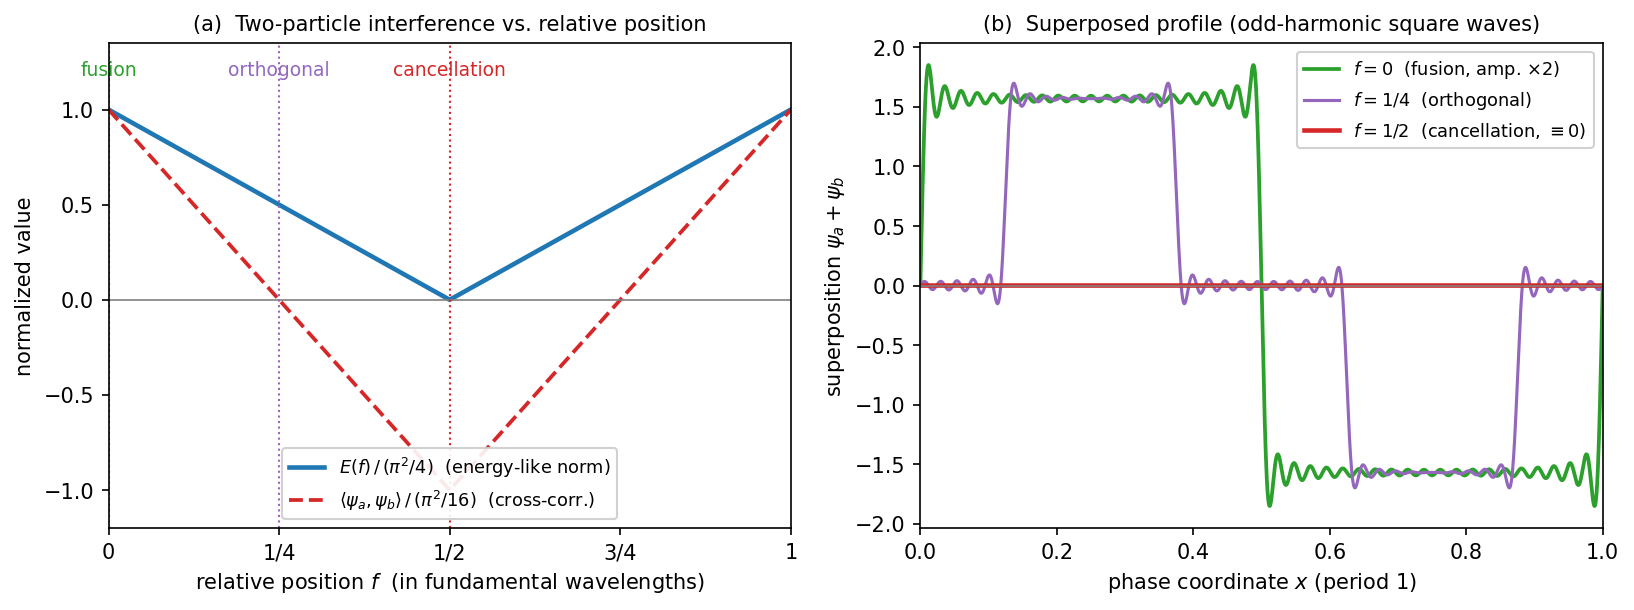
\includegraphics[keepaspectratio,alt={図1}]{p15_interference.png}}
\caption{図1}
\end{figure}

\textbf{図1}：（a）相対位置 \(f\)（基本波長単位）に対する二乗ノルム
\(E(f)\)（三角波・青）と相互相関
\(\langle\psi_a,\psi_b\rangle\)（赤破線）。\(f=0\) で融合、\(f=1/4\)
で直交（相互相関ゼロ）、\(f=1/2\)
で完全打ち消し（\(E=0\)）。（b）重ね合わせプロファイル
\(\psi_a+\psi_b\)（奇数倍音の矩形波・有限項）：\(f=0\)
で振幅二倍、\(f=1/4\) で直交、\(f=1/2\)
で恒等的にゼロ。波形のリンギングは有限項打ち切りによる Gibbs
振動である。

\begin{center}\rule{0.5\linewidth}{0.5pt}\end{center}

\subsection{§5
相対配置の特徴点------融合・直交・完全打ち消し}\label{ux76f8ux5bfeux914dux7f6eux306eux7279ux5fb4ux70b9ux878dux5408ux76f4ux4ea4ux5b8cux5168ux6253ux3061ux6d88ux3057}

相互相関 \(\langle\psi_a,\psi_b\rangle=\dfrac{\pi^2}{16}(1-4f)\)
は、二粒子の関係を端的に表す。これは連続変数 \(f\)
の線形関数であり、\(f\)
自体が離散値しか取れないわけではない。ただしその中に、三つの特徴的な配置（特徴点）が現れる。

\begin{itemize}
\tightlist
\item
  \textbf{\(f=0\)（融合）}：\(\langle\psi_a,\psi_b\rangle\)
  最大。重ね合わせは振幅二倍の単一矩形波になり、二粒子は区別できなくなる（実質一つに見える）。
\item
  \textbf{\(f=\tfrac14\)（直交）}：\(\langle\psi_a,\psi_b\rangle=0\)。二つの矩形波は直交し、干渉のクロス項が消える。\textbf{互いに独立に共存できる}配置であり、区別できる二粒子の自然な置き方である。
\item
  \textbf{\(f=\tfrac12\)（完全打ち消し）}：\(\langle\psi_a,\psi_b\rangle\)
  最小（\(-\pi^2/16\)）。\(\psi_b=-\psi_a\)（矩形波を半周期ずらすと符号反転）となり、\(\psi\equiv0\)。この重ね合わせ規約では合成場が消え、非自明な二粒子モードが残らない。
\end{itemize}

したがって、連続な相対位置 \(f\)
の中に、融合・直交・完全打ち消しに対応する\textbf{離散的な特徴点}が現れる。とりわけ、干渉のクロス項が消えて独立に共存できる直交配置は
\(f=\tfrac14,\tfrac34,\tfrac54,\dots\)（奇数
\(\times\tfrac14\)）に並ぶ離散列を成し、その間隔（ピッチ）は半波長である。融合点（整数
\(f\)）と完全打ち消し点（半整数
\(f\)）のちょうど中間に、直交配置が座る。

ここで「相対位置が離散化される」と言うには、許容配置を直交配置（独立共存）に限る、といった選択原理を別途置く必要がある。本稿はそれを置かず、\(f\)
を連続変数のままとし、その上に直交配置の離散列という特徴点が現れることを観察するに留める。この直交列の間隔（半波長）は、外部に格子があるからではなく、\textbf{粒子自身の広がり（基本波長
\(\propto1/\nu_{R,a}\)、前稿
{[}1{]}）が与えるスケール}である。広がりが小さい（\(\nu_{R,a}\)
が大きい）ほど、直交列の間隔は細かくなる。

なお、これら三つの特徴点のうち、融合（\(f=0\)）・直交（\(f=\tfrac14\)）・完全打ち消し（\(f=\tfrac12\)）の\textbf{存在は矩形波に固有ではなく、半周期符号反転性（奇数倍音のみ）を持つプロファイル一般に普遍}である。実際、一般の奇数倍音プロファイル
\(\sum_{n\ \mathrm{odd}}a_n\sin(2\pi n(x-x_a))\) の相互相関は
\(\tfrac12\sum_{n\ \mathrm{odd}}a_n^2\cos(2\pi n f)\)
であり、\(f=\tfrac14\) ではすべての奇数 \(n\) で \(\cos(n\pi/2)=0\)
となるため、振幅 \(a_n\) に依らず直交する。\(f=\tfrac12\)
での完全打ち消しも半周期符号反転からただちに従う。さらに、各倍音にかかる変調因子
\(\cos(n\pi f)\)（§3
の点2）は二つのコピーのずれから来る幾何的因子であり、振幅 \(a_n\)
に依らない。したがって、どの倍音がどこで消えるか、高次倍音ほど \(f\)
に対して速く間引かれるか、というくし型変調も\textbf{普遍}である。これに対し、その変調を二乗して足し上げた包絡線
\(\sum_{n\ \mathrm{odd}}a_n^2\cos^2(n\pi f)\)
が\textbf{完全な区分線形（三角波）}になることのみが、振幅 \(1/n\)
という矩形波（Walsh 的）選択に固有である（純正弦なら
\(E\propto\cos^2(\pi f)\)
で線形にならない）。したがって、本稿の中心メッセージである三つの特徴点もくし型変調も\textbf{波形選択の任意性から切り離されて頑健}であり、\(E(f)\)
の三角波としての線形包絡線のみが矩形波選択の帰結である。

この振る舞いは、定常波の自己整合条件から離散準位が生じるという既知の構造（定在波による状態の量子化）と\textbf{構造的に対応する}。本稿はこの対応を観察するに留め、量子化の導出を主張しない。

\begin{center}\rule{0.5\linewidth}{0.5pt}\end{center}

\subsection{§6
重なりの可否と量子統計との構造的対応}\label{ux91cdux306aux308aux306eux53efux5426ux3068ux91cfux5b50ux7d71ux8a08ux3068ux306eux69cbux9020ux7684ux5bfeux5fdc}

前節では二粒子を単純に和 \(\psi_a+\psi_b\)
として重ねた。同一の粒子様状態を重ねる際には、和（対称化）か差（反対称化）かという二通りがある。両者で、\textbf{完全な重なり}（\(f=0\)）の可否が反転する。

\textbf{対称結合}
\(\psi_{+}=\psi_a+\psi_b=\displaystyle\sum_{n\ \mathrm{odd}}\frac{2}{n}\cos(n\pi f)\,\sin(2\pi n(x-x_c))\)

\begin{itemize}
\tightlist
\item
  \(f=0\)：\(2\psi_a\)（最大の建設的干渉、振幅二倍）。完全な重なりにおいて\textbf{非自明な合成モードが残る}。これは同じモードに積み上がる振る舞いに対応する。
\item
  \(f=\tfrac12\)：合成場が消える。
\end{itemize}

\textbf{反対称結合}
\(\psi_{-}=\psi_a-\psi_b=\displaystyle\sum_{n\ \mathrm{odd}}\frac{2}{n}\sin(n\pi f)\,\cos(2\pi n(x-x_c))\)

\begin{itemize}
\tightlist
\item
  \(f=0\)：\(\sin(0)=0\) より
  \(\psi_{-}\equiv0\)。\textbf{完全に重ねると合成場が消え、反対称結合としては非自明な二粒子モードを表せない}。
\item
  \(f=\tfrac12\)：\(\sin(n\pi/2)=\pm1\) より最大。
\end{itemize}

すなわち、振幅変調因子が対称結合では \(\cos(n\pi f)\)、反対称結合では
\(\sin(n\pi f)\) となり、\(f=0\)
での可否がちょうど入れ替わる。言い換えれば、

\[\text{「完全に重なれるか」}\ \Longleftrightarrow\ \text{「対称結合か、反対称結合か」}\]

である。完全な重なりが許される対称結合は、同一状態への積み上げを許す振る舞い（ボソン的）を示し、完全に重ねると消える反対称結合は、同一配置の排他（パウリ排他的）に対応する振る舞いを示す。

この対称化／反対称化による重なり可否の分岐は、量子統計におけるボソン／フェルミオンの交換対称性と\textbf{構造的に対応する}。

ただし、ここで扱う \(\psi_\pm=\psi_a\pm\psi_b\) は、単一の関係座標 \(x\)
上での二つのプロファイルの\textbf{一体的な重ね合わせ}であって、二体配置空間
\((x_1,x_2)\) 上の対称化／反対称化
\(\Psi_\pm(x_1,x_2)=\psi_a(x_1)\psi_b(x_2)\pm\psi_a(x_2)\psi_b(x_1)\)（対称
\(\Psi_+\) がボソン、反対称 \(\Psi_-\)
がフェルミ）そのものではない。両者は別の対象である。実際、統計が本来効く一致点
\(f=0\) では、反対称結合の消失は波形に依らない代数的恒等式 \(g-g=0\)
に還元される。したがって、本稿でいう量子統計との「構造的対応」は、\textbf{一致点における代数的消失（\(A-A=0\)）の同型という限定的な意味}での対応であり、二体交換対称性の導出ではない。

また、反対称結合が交換に対して符号反転を伴う点は、閉じた位相上で一周して符号が反転するモード（半整数・二重被覆型）と\textbf{符号反転という形式的共通性}を持つ。ただし、置換群
\(S_2\)
の性質と回転群の位相的性質が非自明に結びつくこと自体がスピン統計定理の深い内容であり、本稿はその結合を主張せず、形式的共通性の指摘に留める。

以上より、本稿の対応は重ね合わせ規約（対称化／反対称化）のレベルでの観察にすぎず、波動関数の対称性とスピンを結ぶスピン統計定理そのものの説明ではない。本稿はこの対応を観察するに留め、量子統計の導出は主張しない。

\begin{center}\rule{0.5\linewidth}{0.5pt}\end{center}

\subsection{§7
振動数が異なる場合（観察）}\label{ux632fux52d5ux6570ux304cux7570ux306aux308bux5834ux5408ux89b3ux5bdf}

ここまでは二粒子の振動数が一致する場合を扱った。振動数が異なる場合を、観察として簡潔に述べる。

ここでは、二つの振動数が共通の周期線上で\textbf{整数モード}として表される場合（または有理比で共通周期が取れる場合）に限って述べる。整数モードどうしの正弦は閉じた区間上で直交する（\(\int_0^1\sin(2\pi m x)\sin(2\pi n x)\,dx=0\),
\(m\neq n\)
整数）。したがって、二粒子の相互相関は\textbf{共有された倍音からのみ}生じる：

\[\langle\psi_a,\psi_b\rangle=\sum_{\omega\,\in\,\text{共有}}\frac{1}{2\,m_\omega\,l_\omega}\cos(2\pi\omega f),\qquad \omega=m\,\nu_a=l\,\nu_b\ (m,l\ \text{odd}).\]

共有倍音が一つも無ければ \(\langle\psi_a,\psi_b\rangle=0\)
となり、相対位置 \(f\)
に依らず干渉は消える。このとき二粒子は任意の相対位置で独立に共存でき、\textbf{配置は自由}になる。

共有の有無は、振動数比の整数構造で決まる。\(\nu_a/\nu_b\) を既約分数
\(r/s\) と書けるとき、両者の奇数倍音ラダー \(\nu_a\{1,3,5,\dots\}\) と
\(\nu_b\{1,3,5,\dots\}\) が共有点を持つのは、\textbf{\(r,s\)
がともに奇数}のときである（このとき \(m s=l r\) を満たす奇数 \(m,l\)
が存在する）。整数振動数に正規化して
\(\nu_a=2^{\alpha}p',\ \nu_b=2^{\beta}q'\)（\(p',q'\)
奇）と分解すれば、これは \(\alpha=\beta\)（\(2\)
の冪成分の一致）に対応する。\(r\) と \(s\)
の偶奇が異なる場合（\(\alpha\neq\beta\)）は、奇数倍音を一切共有せず、完全直交＝自由配置となる。

なお \(\nu_a/\nu_b\) が無理数の場合は、共通周期が存在せず、本稿の「周期
\(1\)
の一本の閉位相線」という設定自体が成立しない。この場合に干渉が消えるという言明は、本設定の外への発見的な外挿であって、本稿の枠内の結論ではない。

まとめると、本稿の枠組みでは次の対応が観察される。

\begin{itemize}
\tightlist
\item
  \textbf{同一振動数（同一粒子）}：全倍音が一致し、§3〜§6
  の強い干渉・鋭い特徴点・統計的振る舞いが現れる。
\item
  \textbf{異なるが整合（奇数比）}：高次倍音のみを共有し（重み
  \(1/(m l)\) が小さい）、弱い干渉・弱い特徴が残る。
\item
  \textbf{非整合（\(2\)
  の冪が異なる）}：干渉が消え、自由配置・独立（無理数比は共通周期を持たず、本設定の外）。
\end{itemize}

これは、交換統計が同一粒子にのみ働き、区別できる粒子には働かないという既知の事実と\textbf{構造的に対応する}。本稿はこの対応を観察するに留める。

\begin{center}\rule{0.5\linewidth}{0.5pt}\end{center}

\subsection{§8
本稿で扱わないこと}\label{ux672cux7a3fux3067ux6271ux308fux306aux3044ux3053ux3068}

本稿は、以下を扱わない。

\begin{itemize}
\tightlist
\item
  一般の \(S^4(R_{\mathrm U})\)
  上での座標不変な相対配置・干渉の定式化（本稿は一次元最小設定に限定する）
\item
  スピン統計定理・ヒルベルト空間構造・場の量子論の導出
\item
  局所モードの安定性・力学（運動方程式・エネルギー汎関数）の判定
\item
  粒子数のゆらぎ・存在の不確定性、仮想粒子との対応
\item
  三体以上の干渉、配置空間の高次元構造
\item
  本稿の干渉構造を具体的な量子数・スペクトル・現実の統計と同定すること
\end{itemize}

これらは、本稿の二粒子干渉という観察をさらに発展させた場合に検討しうる拡張課題である。しかし、現段階では本稿の範囲を超える。

\begin{center}\rule{0.5\linewidth}{0.5pt}\end{center}

\subsection{§9
本稿の主張範囲}\label{ux672cux7a3fux306eux4e3bux5f35ux7bc4ux56f2}

本稿の主張は、次の範囲に限定される。

第一に、閉じた一次元の関係的設定の上で、同一振動数の二つの矩形定常波の重ね合わせのスペクトルは、同じ奇数倍音ラダー上にとどまり、各倍音の振幅は
\(A_n=\tfrac{2}{n}\cos(n\pi f)\) で与えられる。

第二に、その総二乗ノルム（エネルギー様量）は三角波
\(E(f)=\tfrac{\pi^2}{4}(1-2f)\)（\(0\le f\le\tfrac12\)）であり、矩形波の自己相関に等しい。

第三に、連続な相対位置 \(f\) の中に離散的な特徴点が現れ、\(f=0\)
で融合、\(f=\tfrac14\) で直交（独立共存）、\(f=\tfrac12\)
で完全打ち消し（合成場が消え非自明モードが残らない）となる。

第四に、二粒子の重ね合わせを対称化するか反対称化するかに応じて、完全な重なりが許容（ボソン的）または合成場が消える＝排他的（フェルミ的）になる。

第五に、振動数が異なる場合、干渉は共有された奇数倍音からのみ生じ、共有がなければ干渉は消えて自由配置となる。共有の有無は
\(\nu_a/\nu_b\) が奇数比か否か（\(2\) の冪の一致）で決まる。

第六に、以上はすべて既知の構造（定在波の量子化、量子統計の交換対称性）との\textbf{構造的対応の観察}であり、それらの導出ではない。

\begin{center}\rule{0.5\linewidth}{0.5pt}\end{center}

\subsection{まとめ}\label{ux307eux3068ux3081}

本稿の中心的な観察は、次のように要約できる。

\begin{quote}
広がり位相を持つ二つの粒子様状態を、閉じた一次元の関係的設定の上で矩形定常波として重ねると、連続な相対位置の中に離散的な特徴点（融合・直交・完全打ち消し）が現れ、対称化／反対称化に応じて完全な重なりの可否（ボソン的／フェルミ的）が分かれる。これらは初等的なフーリエ級数の閉じた計算として現れる。
\end{quote}

前稿 {[}1{]}
が単一粒子の幾何的舞台と広がりを定めたのに対し、本稿は、その舞台に二粒子を置いたときに現れる関係的構造------相対配置の特徴点と量子統計との構造的対応------を、観察として提示する。なお本稿の計算自体は、周期
\(1\) の閉位相線上の矩形波のフーリエ解析として完結しており、§1
の中心投影・主観幾何 \(S^4(R_{\mathrm U})\)
はその動機づけの枠組みである。一般の \(S^4(R_{\mathrm U})\)
上での座標不変な定式化、三体以上、力学と安定性は、後続稿の主題とする。

\begin{center}\rule{0.5\linewidth}{0.5pt}\end{center}

\subsection{参考文献}\label{ux53c2ux8003ux6587ux732e}

{[}1{]} N. Kihara (2026).
\emph{真空宇宙の中心投影と、広がり位相を持つ粒子様状態}.
観察論文（同著者・前稿）. Concept DOI:
\href{https://doi.org/10.5281/zenodo.20543044}{10.5281/zenodo.20543044}.

{[}2{]} N. Kihara (2026).
\emph{あるモデル粒子をめぐる思考実験（続）------総和ゼロ条件から見る第五の振動数と合成曲率}.
観察論文（同著者）. Concept DOI:
\href{https://doi.org/10.5281/zenodo.20535894}{10.5281/zenodo.20535894}.

{[}3{]} N. Kihara (2026). \emph{球面投影 \(\sigma_R\)（radial
projection）の定義------中心投影シリーズの基礎写像}. 観察論文（同著者）.
Concept DOI:
\href{https://doi.org/10.5281/zenodo.20462569}{10.5281/zenodo.20462569}.

{[}4{]} T. W. Körner (1988). \emph{Fourier Analysis}. Cambridge
University Press.（矩形波のフーリエ級数、Parseval
の関係、自己相関と三角波）

（注：外部参照は Concept DOI を用いる。）

\begin{center}\rule{0.5\linewidth}{0.5pt}\end{center}

\subsection{改訂履歴}\label{ux6539ux8a02ux5c65ux6b74}

\begin{itemize}
\tightlist
\item
  \textbf{v1.0（2026-06）}：初版（公開候補）。前稿 {[}1{]}
  が後続稿に委ねた複数粒子の干渉のうち、最小の場合（同一振動数の二粒子、閉じた一次元設定）を扱う。同一倍音の重ね合わせのスペクトル
  \(A_n=\tfrac{2}{n}\cos(n\pi f)\)、三角波の二乗ノルム
  \(E(f)=\tfrac{\pi^2}{4}(1-2f)\)（矩形波の自己相関）、連続な相対位置の中に現れる離散的な特徴点（融合
  \(f{=}0\)・直交 \(f{=}\tfrac14\)・完全打ち消し
  \(f{=}\tfrac12\)）、対称／反対称化による重なり可否の反転（ボソン的／フェルミ的）、異振動数では共有倍音の有無（既約比
  \(r/s\) がともに奇数＝\(2\)
  の冪成分の一致）が干渉を支配することを、いずれも構造的対応の観察として提示。外部査読（ChatGPT・Grok・Gemini）を反映：「離散化」を「離散的な特徴点の出現」、「禁止」を「完全打ち消し／非自明モードが残らない」、「統計の創発」を「量子統計との構造的対応」に弱め、\(E(f)\)
  を物理的エネルギーでなく Parseval
  二乗ノルムに基づくエネルギー様量と明記、矩形波を関係位相座標上の大域的定常プロファイル（局在波束ではない）と明記、§7
  を整数モード／有理比に限定して厳密化。§2
  に矩形波採用の機能的理由（波高に物理的意味を与えない・形状決定は後続に委ねる）を最小限追記。§6
  に「本稿の対応は重ね合わせ規約のレベルの観察にすぎず、スピン統計定理そのものの説明ではない」を明記。\(E(f)\)
  の三角波・相互相関の特徴点（\(f=0,1/4,1/2\)）と重ね合わせ波形を可視化した図1を
  §4 に追加。さらに外部査読（Claude.ai）を反映：(a) §6
  に、\(\psi_\pm=\psi_a\pm\psi_b\)
  は一体の重ね合わせであって二体配置空間 \((x_1,x_2)\)
  上の反対称化そのものではないこと、対応は一致点での代数的消失 \(A-A=0\)
  の同型という限定的意味であることを明記、二重被覆との関係を「符号反転の形式的共通性の指摘に留める」に弱化。(b)
  §5
  に、三つの特徴点（融合・直交・完全打ち消し）の存在は半周期符号反転性を持つ波形一般に普遍で、三角波の線形性のみが矩形波選択に固有である旨を追記（波形依存／普遍の切り分け）。(c)
  §4 に、相互相関の線形式が \([0,\tfrac12]\)
  の枝であること、本稿の「干渉」が静的な重なり積分であることを注記。(d)
  §7
  で無理数比を「共通周期を持たず本設定の外」と位置づけ。スピン統計定理・量子統計の導出は主張せず、一般の
  \(S^4\) 上の定式化・力学・三体以上は後続稿に委ねる。
\end{itemize}

\end{document}
